
\section{Data and Synthetic}

Considered Data for conducting this study contains thirty moderate-magnitude earthquakes ($3.5 > M_w > 5.5$) occurred between 1998 and 2014. The latest version of ground motion prediction equations (GMPEs) database includes small-to-moderate earthquakes in California which will be helpful in calibration of compariosion criteria. 
Selected events are spread throughout a simulation domain with a volume projection of \vdomain{180}{135}{62}{km}, which covers the entire Los Angeles metropolitan area and most of the significant geologic structures around. Fig.~\ref{fig:region} shows the simlation domain in which we labled the events with sequential letter code from A to Z and AA to AD and Table \ref{tab:events} provides detailed information for those selected events.The unprocessed recorded data from Southern California Earthquake Data Center (SCEDC) and Center for Engineering Strong Motion Data (CESMD) are downloaded for each of the earthquakes to take advantage of the numerous time series available from different data centers. We obtained records for moree than 800 stations, Some of which were in common between different networks and some were not usable. Records from SDEDC and CESMD were processed and selected for each event. we performed gain and baseline corrections, and applied a high-pass filter at 0.05 Hz before integrating to obtain velocities and displacements. The final number of chosen records for validation for any of the selected earthquake can be found in Table \ref{tab:events}.

\begin{figure*}
    \centering
    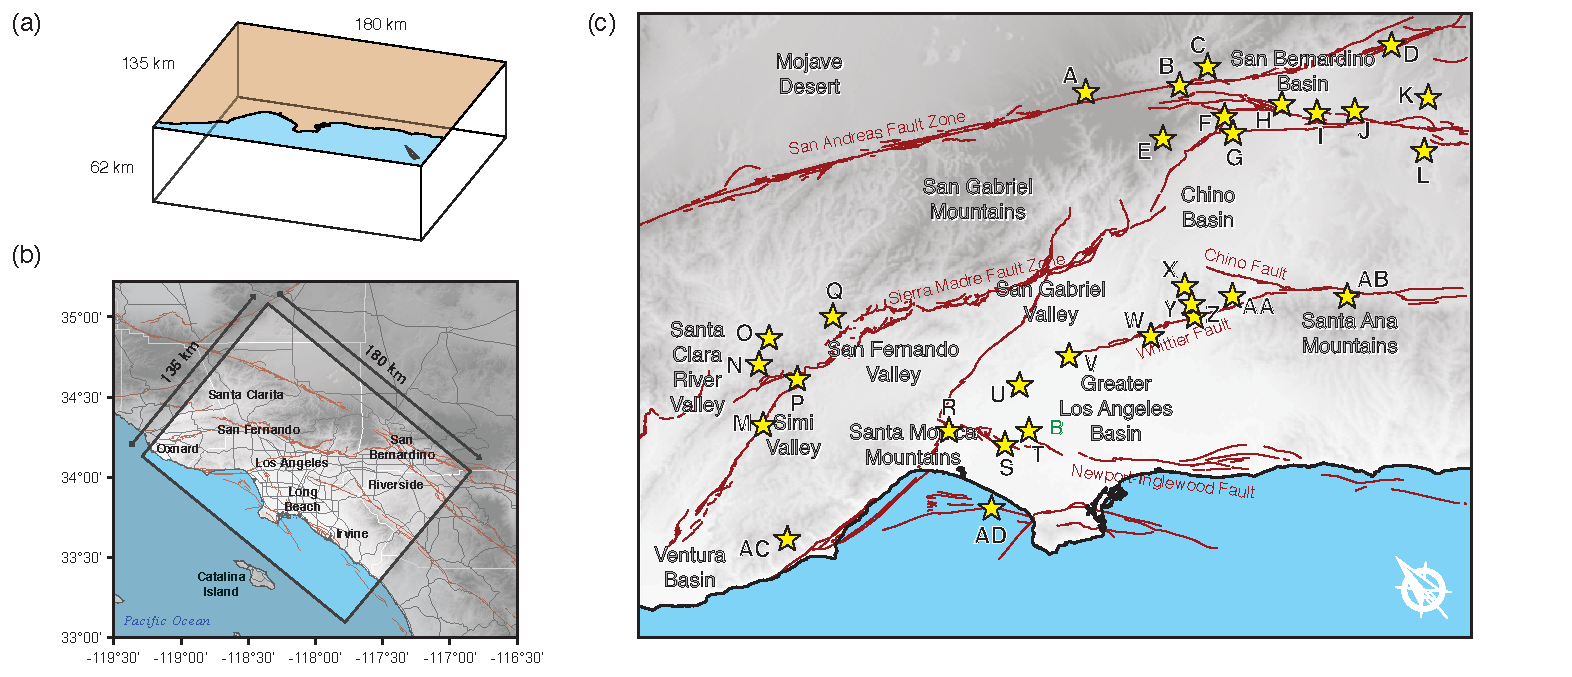
\includegraphics
    	[width=\textwidth]
    	{figures/pdf/figure-01}
    \caption{Region of interest and simulation domain. (a) 3D view of the simulation domain. (b) Geographical location and surface projection of the simulation domain, along with the names of the main cities surrounding the Los Angeles metropolitan are. (c) Major geologic structures including basins, valleys and mountains, along with the main quaternary faults in the region. The color background represents the surface \vsthirty{} values included in the CVM-H+GTL model, with a topography shading effect.}
    \label{fig:region}
\end{figure*}

\input{tab-earthquakes}

The simulations of the selected events are all done for the four major velocity models currently available for the region of southern California: CVM-S4, CVM-S4.26, CVM-H and CVM-H+GTL. 3D simulations with point source model are done at maximum frequency of 1 Hz and minumum shear wave velocity of 200 m/s for each earthquake and velocity model combination using Hercules, a parallel 3D finite element computer application for solving forward anelastic wave propagation problems which has been thoroughly tested and verified in multiple supercomputers. All the runs are done on Blue Waters at the National Center for Supercomputing Applications.

Using a developed python code, we collect the results of the Peak Ground Acceleration (PGA), Peak Ground Velocity (PGV), and Peak Ground Displacement (PGD) in three directions (EW, NS, Up), for all the events in all available stations for both synthetics and data. This information will be used later in validation method.
